
\subsection{RL agent} \label{sec:methods_rl_agent}

\paragraph{Learning algorithm.} 

We use Muesli ~\citep{hessel2021muesli} as our RL algorithm. We briefly describe the algorithm here, but refer the reader to the original publication for details. Taking a history-dependent encoding as input, in our case the output of an RNN or Transformer, AdA learns a sequence model (an LSTM) to predict the values $\hat{v_i}$, action-distributions $\hat{\pi_i}$ and rewards $\hat{r_i}$ for the next $I$ steps. Here, $i = 0, \dots, I$ denotes the prediction $i$ steps ahead. $I$ is typically small and in our case $I = 4$. For each observed step $t$, the model is unrolled for $I$ steps and updated towards respective targets: \begin{equation}
\mathcal{L}_r^t=\sum_{i=0}^I\left(\hat{r}^t_i - r_{t+i}\right)^2, \; \mathcal{L}_v^t=\sum_{i=0}^I\left(\hat{v}^t_i - G_{t+i}\right)^2, \; \mathcal{L}_{\pi}^t=\sum_{i=0}^I \textrm{KL}\left(\left. \left. \pi^{t+i}_{\textrm{CMPO}} \ \right|\right|\  \hat{\pi}^t_i \right).\label{eq:muesli_losses}
\end{equation}
Here, $r_{t+i}$ refers to the observed rewards. $G_{t+i}$ refers to value-targets which are obtained using Retrace~\citep{munos2016safe} based on Q-values obtained from one-step predictions of the model.

The action-targets $\pi^{t}_{\textrm{CMPO}}$ are obtained by re-weighting the current policy\footnote{The prior distribution is actually a mixture of the current estimate of the policy, the (outdated) policy used to produce the sample and the uniform distribution where the latter two are mixed in as regularisers.} using clipped, normalised, exponentially transformed advantages. Muesli furthermore incorporates an additional auxiliary policy-gradient loss based on these advantages to help optimise immediate predictions of action-probabilities. Finally, Muesli maintains a target network which trails the sequence model and is used for acting and to compute Retrace targets and advantages.

\begin{figure}
    \centering
    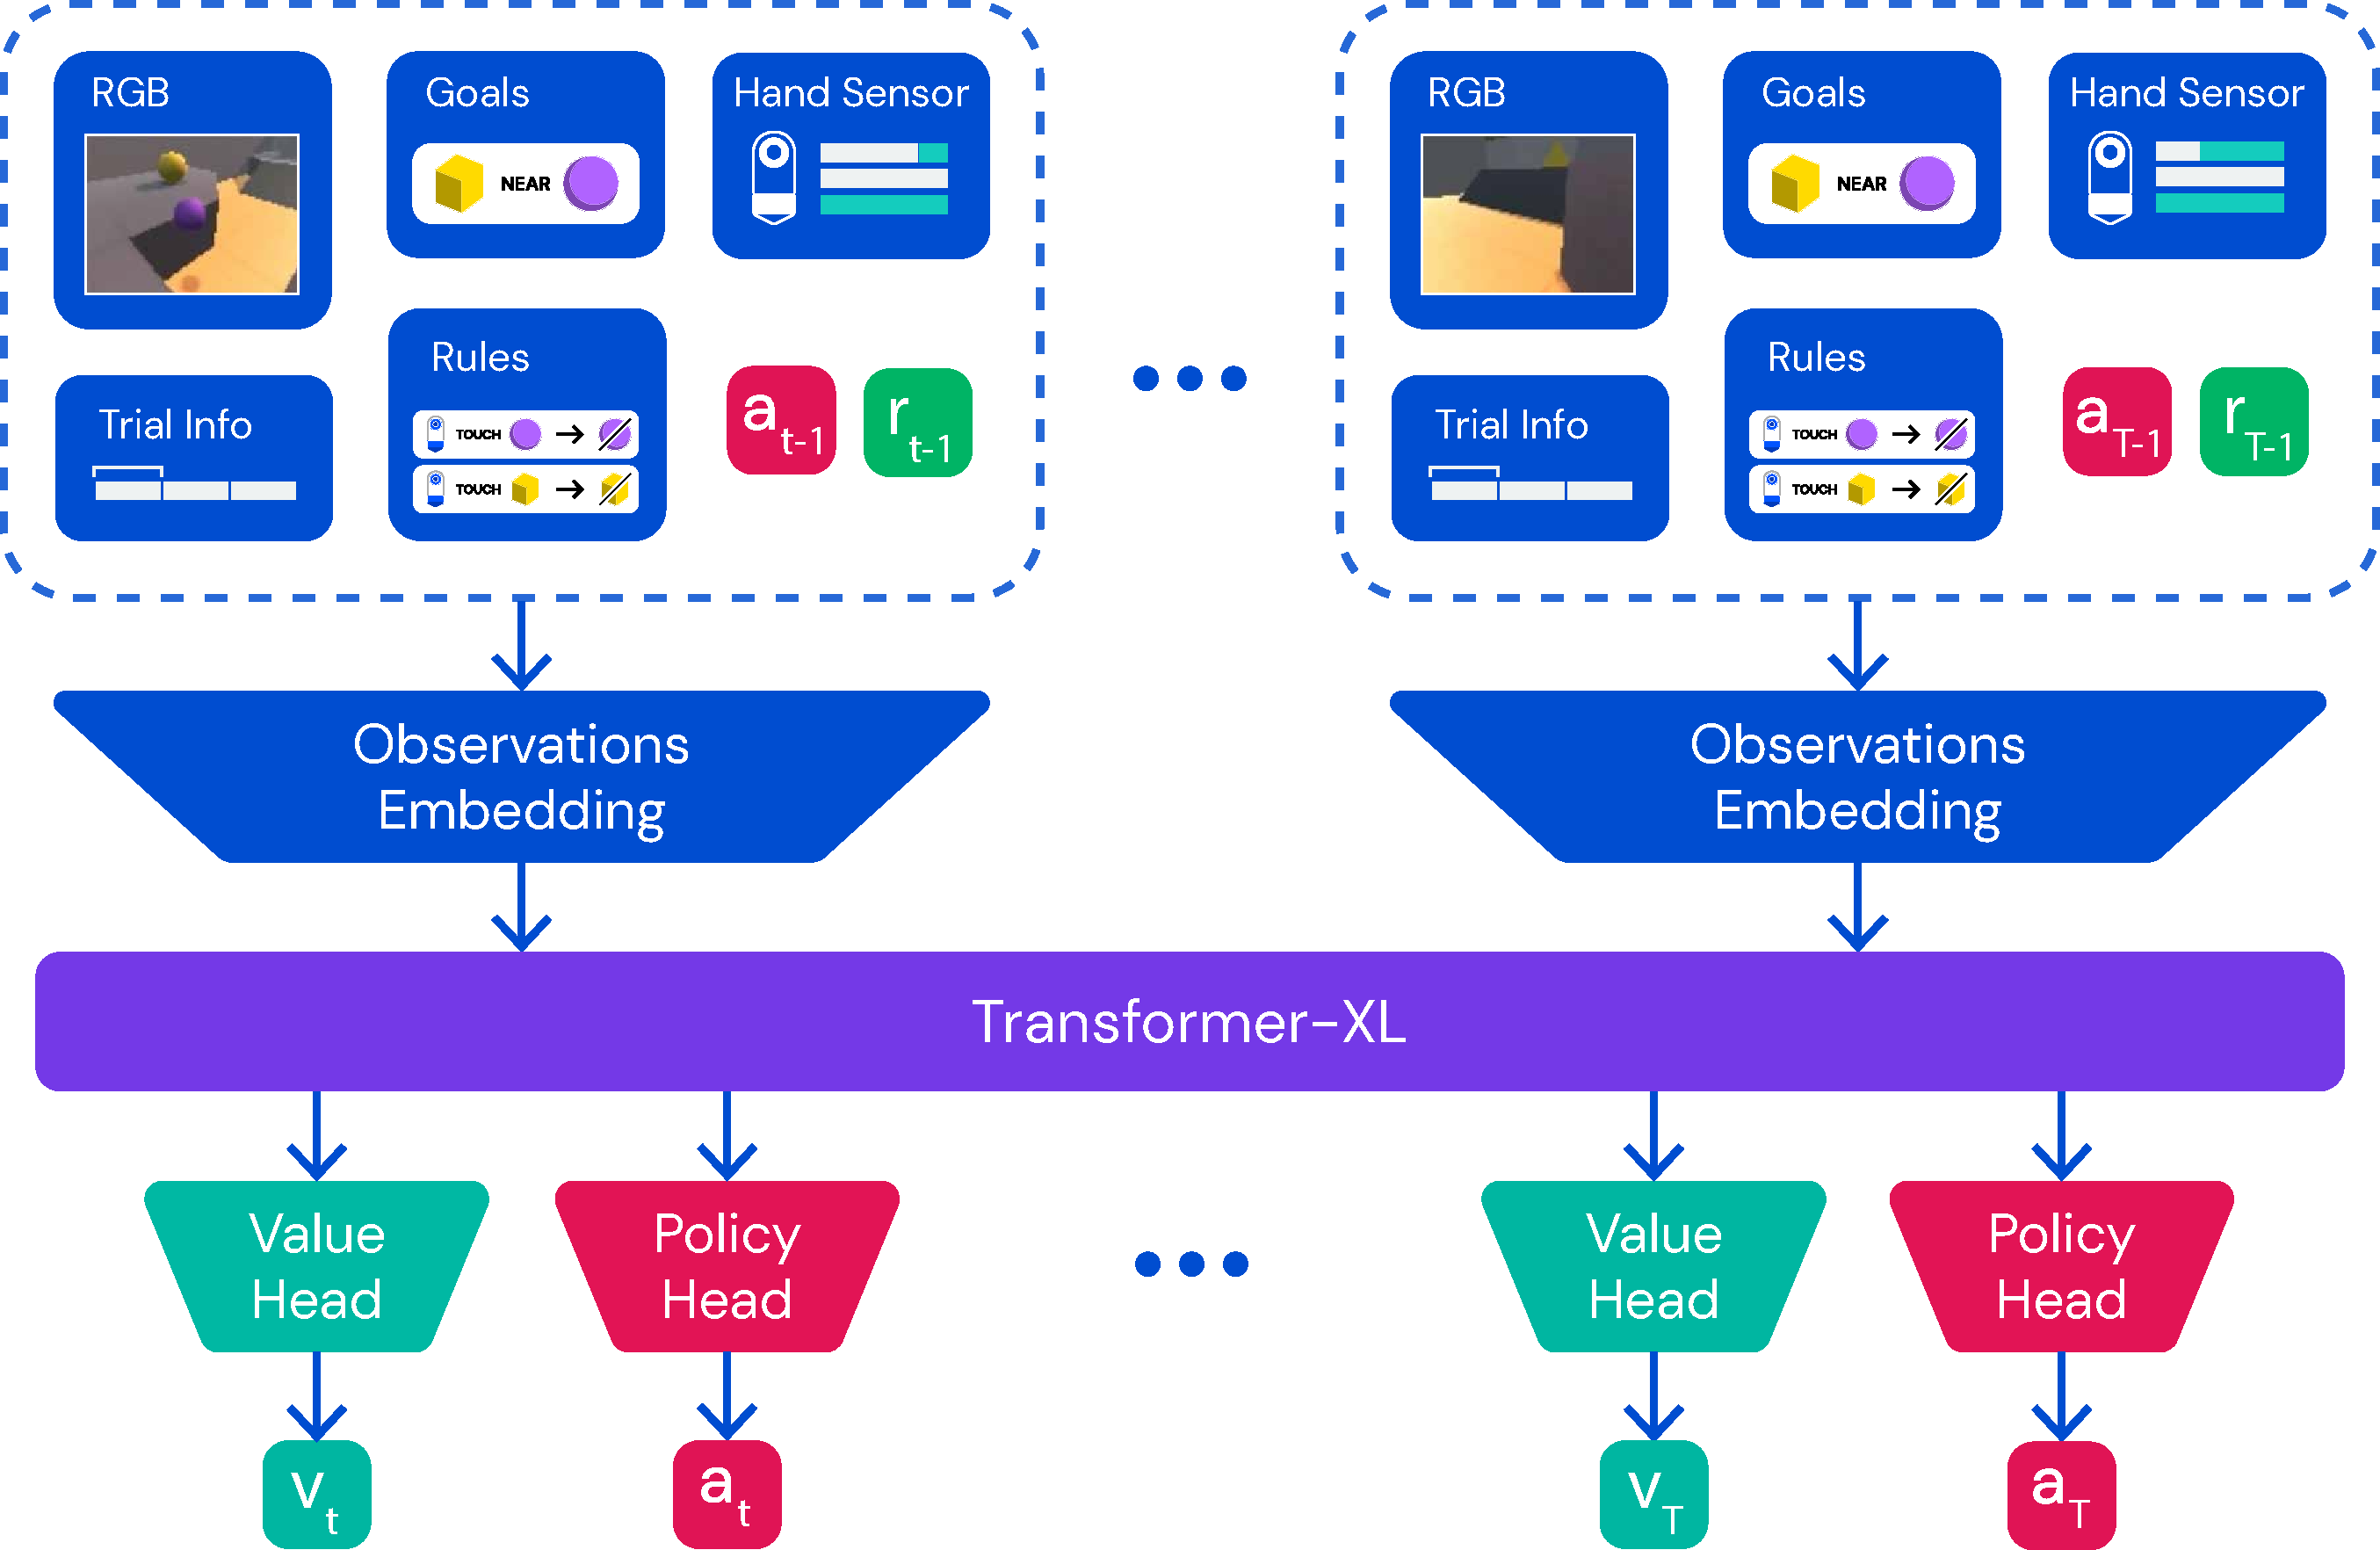
\includegraphics[width=0.7\textwidth]{figures/ada_paper_diagrams_transformer.pdf}
    \caption{\textbf{Agent architecture.} For each timestep, we embed and combine the pixel observation, goal, hand, trial and time information, production rules, previous action, and previous reward into a single vector. These observations embeddings pass in sequence to the Transformer-XL, whose output embeddings feed into an MLP value head, MLP policy head, and the Muesli LSTM model step (omitted in the diagram for brevity). See Appendix \ref{app:agent-architecture} for more details about our agent architecture.}
    \label{fig:transformer_viz}
\end{figure}

\paragraph{Memory architecture.} 
\label{sec:memory-architectures}
Memory is a crucial component for adaptation as it allows the agent to store and recall information learned and experienced in the past. In order for agents to effectively adjust to the changes in task requirements, memory should allow the agent to recall information from both the very recent and the more distant past. While slow gradient-based updates are able to capture the latter, they are often not fast enough to capture the former, i.e. fast adaptation. The majority of work on memory-based meta-RL has relied on RNNs as a mechanism for fast adaptation \citep{parisotto2021meta}. In this work, we show that RNNs are not capable of adaptation in our challenging partially-observable embodied 3D task space. We experiment with two memory architectures to address this problem:

\begin{enumerate}\setlength{\itemsep}{6pt}
\item \emph{RNN with Attention} stores a number of past activations (in our case 64) in an episodic memory and attends over it, using the current hidden state as query. The output of the attention module is then concatenated with the hidden state and fed into the RNN. We increase effective memory length of the agent by storing only every 8\textsuperscript{th} activation in its episodic memory.\footnote{We arrived at these numbers as a compromise between performance and speed. Note that the resulting architecture is slower than an equivalently sized Transformer.}
\item \emph{Transformer-XL (TXL)} \citep{dai2019transformer} is a variant of the Transformer architecture \citep{vaswani2017attention} which enables the use of longer, variable-length context windows to increase the model's ability to capture long-term dependencies. To increase the stability of training Transformers with RL, we follow \citet{parisotto2020stabilizing} in performing  normalisation \textit{before} each layer, and use gating on the feedforward layers as in \citet{shazeer2020glu}.
\end{enumerate}

Both memory modules operate on a sequence of learned timestep embeddings, and produce a sequence of output embeddings that are fed into the Muesli architecture, as shown in Figure \ref{fig:transformer_viz} with a Transformer-XL module. In Section \ref{sec:results_architecture} we show that both attention-based memory modules significantly outperform a vanilla RNN in tasks that require adaptation. Transformer-XL performs the best and therefore is used as the default memory architecture in all our experiments unless stated otherwise. 

\textbf{Going beyond few shots.} We propose a simple modification to our Transformer-XL architecture to increase the effective memory length without additional computational cost. Since observations in visual RL environments tend to be highly temporally correlated, we propose sub-sampling the sequence as described for RNN with Attention, allowing the agent to attend over 4 times as many trials. To ensure that observations which fall between the sub-sampled points can still be attended to, we first encode the entire trajectory using an RNN with the intention of summarising recent history at every step. We show that the additional RNN encoding does not affect the performance of our Transformer-XL variant but enables longer range memory (see Section \ref{sec:results_few_to_many_shot}). 

\subsection{Distillation} \label{sec:methods_distillation}

For the first four billion steps of training, we use an additional distillation loss~\citep{Schmidhuber1992distillation, schmitt2018kickstarting, czarnecki2019distilling} to guide AdA's learning with the policy of a pre-trained teacher, in a process known as kickstarting; iterating this process leads to a generational training regime~\citep{xland,wang2102alchemy}. The teacher is pre-trained from scratch via RL, using an identical training procedure and hyperparameters as AdA, apart from the lack of initial distillation and a smaller model size (23M Transformer parameters for the teacher and 265M for multi-agent AdA). Unlike aforementioned prior work, we do not employ shaping rewards or Population Based Training (PBT,~\citet{jaderberg2017population}) in earlier generations. During distillation, AdA acts according to its own policy and the teacher provides target logits given the trajectories observed by AdA. Distillation allows us to amortise an otherwise costly initial training period, and it allows the agent to overcome harmful representations acquired in the initial phases of training; see Section \ref{sec:results_kickstarting}. 

To integrate the distillation loss with Muesli, we unroll the model from every transition observed by the student. We minimise the KL-divergence between all of the action-probabilities predicted by the model and the action-probabilities predicted by the teacher's policy at the corresponding timestep. Analogously to Muesli's policy-loss $\mathcal{L}_\pi$ defined in \eqref{eq:muesli_losses}, we define
\begin{equation}
\mathcal{L}_{\textrm{dist}}=\sum_{i=0}^I \textrm{KL}\left(\left. \left.\tilde{\pi}^{t+i}_0 \ \right|\right|\ \hat{\pi}^t_i \right)\, ,
\end{equation}
where $\tilde{\pi}$ corresponds to the predicted action-logits provided by the teacher given the same observed history. Furthermore, we found it useful to add additional $L^2$ regularisation during distillation.

\begin{figure}[htb]
    \centering
    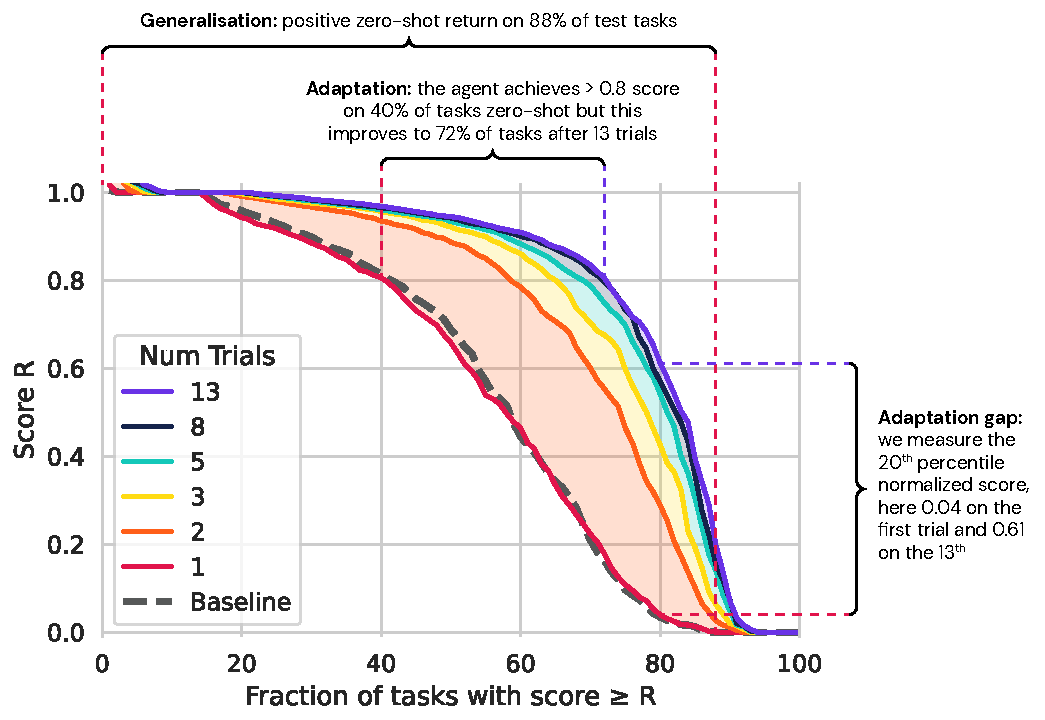
\includegraphics[width=0.8\linewidth]{figures/single_agent_percentiles.pdf}
    \caption{\textbf{Zero-shot generalisation and few-shot adaptation.} We report the distribution of normalised task scores over the single-agent test set when evaluated with various numbers of trials. On the $y$-axis is the total last-trial reward relative to that of an agent fine-tuned on the test tasks (approximating ``infinite trials'' performance). Curves moving further towards the top right corner indicate better performance. When given more trials, the agent achieves higher scores in the last trial, showing test-time adaptation across most of the task distribution (shaded regions). The dashed line indicates the zero-shot performance of an agent trained in a regime where every episode consists of only a single trial.}
    \label{fig:single_agent_percentiles}
\end{figure}

